\documentclass[zihao=-4, a4paper]{ctexart} % 正文小四

% === 宏包引入 ===
\usepackage{geometry}       % 页面边距设置
\usepackage{graphicx}       % 图片支持
\usepackage{amsmath}        % 数学公式
\usepackage{amssymb}        % 数学符号
\usepackage{float}          % 图片浮动控制
\usepackage{booktabs}       % 三线表
\usepackage{subfigure}      % 子图支持
\usepackage{listings}       % 代码块
\usepackage{xcolor}         % 颜色支持
\usepackage{fontspec}       % 字体设置
\usepackage{titlesec}       % 标题格式
\usepackage{titling}        % 标题宏包
\usepackage{ulem}           % 下划线支持
\usepackage{setspace}       % 行间距
\usepackage{caption}        % 图表标题设置
\usepackage{array}          % 表格列格式

% === 字体设置 ===
% 必须使用 XeLaTeX 编译
\setmainfont{Times New Roman} % 字母数字 Time New Roman
\setCJKmainfont[AutoFakeBold=true]{SimSun} % 中文字体 宋体

% === 页面设置 ===
\geometry{left=2.5cm, right=2.5cm, top=2.5cm, bottom=2.5cm}
\onehalfspacing             % 1.5倍行距

% === 章节标题格式设置 ===
\ctexset{
	section = {
		name = {第, 章：}, % 格式：第一章：必要介绍
		number = \chinese{section},
		format = \centering\heiti\zihao{3}, % 三号 黑体 居中
		aftername = {},
		beforeskip = 12pt,
		afterskip = 12pt
	},
	subsection = {
		format = \heiti\zihao{4}, % 小四 黑体
		beforeskip = 6pt,
		afterskip = 6pt
	},
	subsubsection = {
		format = \heiti\zihao{-4} % 小四 黑体
	}
}

% === 代码块样式 ===
\definecolor{codegreen}{rgb}{0,0.6,0}
\definecolor{codegray}{rgb}{0.5,0.5,0.5}
\definecolor{codepurple}{rgb}{0.58,0,0.82}
\definecolor{backcolour}{rgb}{0.95,0.95,0.92}

\lstset{
	backgroundcolor=\color{backcolour},   
	commentstyle=\color{codegreen},
	keywordstyle=\color{magenta},
	numberstyle=\tiny\color{codegray},
	stringstyle=\color{codepurple},
	basicstyle=\ttfamily\footnotesize, % 代码字体稍小
	breakatwhitespace=false,         
	breaklines=true,                 
	captionpos=b,                    
	keepspaces=true,                 
	numbers=left,                    
	numbersep=5pt,                  
	showspaces=false,                
	showstringspaces=false,
	showtabs=false,                  
	tabsize=2,
	language=Matlab,
	frame=single
}

% === 文档开始 ===
\begin{document}
	
	% === 封面 ===
	\begin{titlepage}
		\centering
		\vspace*{0.5cm}
		
		% 校徽
		
\includegraphics[width=8cm]{logo.png} \\[1.2cm]
		
		{\zihao{1}\heiti 傅里叶分析和小波分析期末大作业} \\[1.8cm]
		
		\zihao{3}
		\textbf{题目：} \underline{\makebox[10cm][c]{基于改进 DWT-SVD 与 HVS 自适应机制的}} \\
		\vspace{0.2cm}
		\underline{\makebox[11.5cm][c]{数字图像盲水印算法鲁棒性深度研究报告}} \\[1.5cm]
		
		\zihao{4}
		\textbf{理} \underline{\makebox[2cm][c]{}} \textbf{学院} \quad 
		\textbf{信息与计算科学} \underline{\makebox[2cm][c]{}} \textbf{专业} \\[1cm]
		
		\begin{tabular}{rc}
			\textbf{学 \quad \quad 号} & \underline{\makebox[6cm][c]{1043220122}} \\[0.6cm]
			\textbf{学生姓名} & \underline{\makebox[6cm][c]{林鑫}} \\
		\end{tabular}
		
		\vspace{2cm}
		{\zihao{4} 二〇二五 年 十二 月}
	\end{titlepage}
	
	% === 摘要 ===
	\thispagestyle{plain}
	\begin{center}
		\heiti\zihao{3} 摘 \quad 要
	\end{center}
	
	\vspace{1em}
	\noindent
	随着多媒体技术的飞速发展和互联网的普及，数字图像的版权保护、内容认证及防篡改需求日益迫切[1]。数字水印技术作为一种有效的信息隐藏手段，已成为信息安全领域的研究热点。传统的基于离散小波变换（DWT）的水印算法虽然在时频局部化方面优于离散余弦变换（DCT）和离散傅里叶变换（DFT），但在面对几何攻击（如旋转、缩放）和严重信号处理攻击（如强压缩、滤波）时，往往表现出鲁棒性不足的缺陷。
	
	为了克服单一变换域的局限性，本报告提出并详细论证了一种基于 DWT 与奇异值分解（SVD）相结合的混合盲水印算法，并引入 Arnold 置乱加密与基于人类视觉系统（HVS）的自适应嵌入强度策略。本研究通过深入的理论分析与模拟实验对比，揭示了混合域算法在不可感知性与鲁棒性平衡上的显著优势，特别是针对 DWT 固有的几何脆弱性问题提供了基于奇异值稳定性的解决方案，为高水平的大作业设计提供了详尽的理论依据与实施路径。
	
	\vspace{1em}
	\noindent \textbf{关键词：} 数字水印；DWT-SVD；HVS；Arnold置乱；鲁棒性
	
	% === 正文内容 ===
	
	\section{必要介绍}
	
	\subsection{研究背景与意义}
	在数字化时代，多媒体数据的复制与传播变得异常便捷，但这同时也带来了严峻的版权侵权与数据篡改风险。数字水印技术应运而生，它通过将特定的标识信息（水印）隐蔽地嵌入到数字媒体（宿主）中，以证明所有权或验证内容的完整性。与传统的加密技术不同，加密仅在传输过程中保护数据，一旦解密，数据即失去保护；而数字水印则能与内容永久结合，提供全生命周期的保护。
	
	在学术界与工业界的共同推动下，数字水印算法经历了从空域（Spatial Domain）到变换域（Transform Domain）的演进。早期的空域算法如最低有效位（LSB）替换法，虽然计算简单且容量大，但鲁棒性极差，简单的图像处理即可破坏水印。随后的变换域算法，利用 DCT、DFT 等工具将图像能量分散，显著提高了抗压缩能力。然而，随着攻击手段的复杂化，特别是几何变换攻击和混合攻击的出现，单一变换域算法逐渐显露出瓶颈。
	
	本研究的意义在于，针对现有 DWT 算法的局限性，通过引入 SVD 的代数特征稳定性和 HVS 的感知掩蔽特性，构建一种不仅对常规信号处理鲁棒，且对几何失真具有一定抵抗力的“混合域”水印方案。这不仅是对经典理论的验证，更是对高阶信号处理技术在信息安全中应用的深入探索。
	
	\subsection{问题提出与实验动机}
	传统的单一 DWT 算法虽具备良好的时频特性，但在几何攻击下往往失效。本研究旨在通过引入 SVD 的代数特征稳定性，解决常规压缩与剪切攻击的问题，并通过实测数据验证其在旋转与噪声攻击下的真实性能边界。
	
	\subsection{本报告的研究目标与方案升级}
	为了解决上述问题并确保大作业的高分产出，本报告提出将原方案升级为“基于 DWT-SVD 的自适应盲水印算法”。主要改进点如下：
	\begin{itemize}
		\item \textbf{混合变换域}：结合 DWT 的时频分解能力与 SVD 奇异值的稳定性，提高对信号处理和几何攻击的鲁棒性。
		\item \textbf{混沌加密}：引入 Arnold 变换对水印进行预处理置乱，提升安全性并分散错误比特。
		\item \textbf{HVS 自适应}：利用分块方差计算局部纹理复杂度，动态调整嵌入强度，实现不可感知性与鲁棒性的最佳平衡。
	\end{itemize}
	
	\section{实验原理}
	
	\subsection{离散小波变换（DWT）的多分辨率分析}
	DWT 是通过尺度函数和小波函数对信号进行多尺度分解的工具。对于二维图像信号 $I(x, y)$，DWT 通过行和列的一维滤波与下采样，将图像分解为四个子带：
	\begin{itemize}
		\item LL（低频逼近）：包含图像的主要能量和轮廓信息。
		\item HL（水平细节）：保留水平方向的边缘信息。
		\item LH（垂直细节）：保留垂直方向的边缘信息。
		\item HH（对角细节）：包含高频噪声和对角线边缘。
	\end{itemize}
	数学上，一级分解可表示为：
	\begin{equation}
		I(x,y) \xrightarrow{\text{DWT}} \{LL_1, LH_1, HL_1, HH_1\}
	\end{equation}
	为了获得更好的频率分离度，通常对 $LL_1$ 进行二级分解得到 $\{LL_2, LH_2, HL_2, HH_2\}$。
	
	\textbf{理论洞察}：
	人眼视觉系统（HVS）对低频信息极其敏感，任何对 $LL$ 子带的修改都极易引起可察觉的失真；而 $HH$ 子带虽不易被察觉，但极易被 JPEG 压缩（高频量化）滤除[11]。因此，选择中频子带（$HL_2$ 或 $LH_2$）作为水印嵌入域是平衡“鲁棒性”与“不可感知性”的最佳选择。此外，选用 db4 (Daubechies-4) 小波基相比 Haar 小波具有更长的滤波器长度和更好的能量聚集性，能减少重构时的块效应。
	
	\subsection{奇异值分解（SVD）的稳定性原理}
	奇异值分解是线性代数中的核心技术。对于任意图像块矩阵 $A$（大小 $N \times N$），SVD 将其分解为：
	\begin{equation}
		A = U S V^T
	\end{equation}
	其中，$U$ 和 $V$ 是正交矩阵 ($U^T U = I, V^T V = I$)，$S$ 是对角矩阵，对角线元素 $\lambda_i$ 即为奇异值，且 $\lambda_1 \ge \lambda_2 \ge \dots \ge \lambda_N \ge 0$。
	
	\textbf{SVD 在水印中的核心优势}：
	\begin{itemize}
		\item \textbf{极高的稳定性}：当图像受到微小的扰动（如加噪、滤波、轻微压缩）时，其奇异值 $\lambda_i$ 的变化非常微小。这意味着将水印信息嵌入到奇异值中，比直接修改像素值或小波系数具有更强的抗攻击能力。
		\item \textbf{内蕴代数特征}：奇异值代表了图像块的内蕴能量分布，与图像的几何位置耦合度较低（相对于直接像素映射），因此对几何变换具有一定的抵抗力。
		\item \textbf{转置不变性}：$A$ 与 $A^T$ 具有相同的非零奇异值，这意味着 SVD 水印天然具有抗转置（翻转）攻击的能力。
	\end{itemize}
	
	\subsection{混沌动力学与 Arnold 置乱}
	为了消除水印像素间的空间相关性，并提高安全性，采用 Arnold 变换（猫映射）对二值水印图像进行置乱。其二维映射公式为：
	\begin{equation}
		\begin{bmatrix} x' \\ y' \end{bmatrix} = \begin{bmatrix} 1 & 1 \\ 1 & 2 \end{bmatrix} \begin{bmatrix} x \\ y \end{bmatrix} \pmod N
	\end{equation}
	其中 $(x,y)$ 是原始像素坐标，$(x',y')$ 是变换后坐标，$N$ 是图像尺寸。
	
	\textbf{周期性与密钥}：
	Arnold 变换具有周期性，即经过 $T$ 次迭代后图像会恢复原状。迭代次数 $k (k < T)$ 作为密钥。如果攻击者截获了含水印图像并试图提取，在不知道 $k$ 的情况下，提取出的仅是杂乱无章的噪声。
	对于 $N=64$ 的图像，周期 $T=48$。
	对于 $N=128$ 的图像，周期 $T=96$。
	这种置乱不仅保护了信息，还在遭受裁剪攻击时发挥关键作用：局部裁剪导致的噪声在反置乱后会弥散到整个水印图像中，使得整体轮廓依然可辨，而非局部彻底缺失。
	
	\subsection{HVS 感知掩蔽模型与自适应强度}
	人眼对图像不同区域的噪声敏感度由“刚好可察觉差异”（Just Noticeable Difference, JND）决定。HVS 模型指出：
	\begin{itemize}
		\item \textbf{亮度掩蔽}：人眼对极亮或极暗区域的噪声不敏感。
		\item \textbf{纹理掩蔽}：在纹理复杂（方差大、熵高）的区域，人眼很难察觉额外的噪声。
	\end{itemize}
	基于此，本研究摒弃固定嵌入强度 $\alpha$，采用基于局部块方差的自适应强度计算公式：
	\begin{equation}
		\alpha_i = \alpha_{min} + \beta \cdot \log(1 + Var(B_i))
	\end{equation}
	其中 $Var(B_i)$ 是当前图像块的方差，$\alpha_{min}$ 是基础强度，$\beta$ 是调节系数。这确保了在平坦区域使用较小的 $\alpha$ 以保证不可见性，在纹理区域使用较大的 $\alpha$ 以提升鲁棒性。
	
	\section{实验过程}
	
	\subsection{总体架构}
	本研究设计的系统分为三个主要模块：水印预处理、嵌入过程和盲提取过程。
	
	\subsection{模块一：水印预处理}
	输入：二值水印图像 $W$ (尺寸 $64 \times 64$)。
	置乱：设定密钥 $Key = K$ (例如 $K=10$)，应用 Arnold 变换公式迭代 $K$ 次，得到置乱后的水印 $W_{scr}$。
	向量化：将二维矩阵 $W_{scr}$ 转换为一维向量 $V_w$，便于后续逐位嵌入。
	
	\subsection{模块二：水印嵌入算法 (DWT-SVD + HVS)}
	该过程是核心创新点，结合了频域分解与代数特征修改。
	
	\textbf{步骤 1：宿主图像分解}
	读取宿主图像 $I (512 \times 512)$，利用 db4 小波进行 2 级 DWT 分解。提取二级水平细节子带 $HL_2$（尺寸 $128 \times 128$）。选取 $HL_2$ 是因为它包含丰富的纹理信息，适合 HVS 掩蔽，且比 $HH_2$ 更抗压缩[11]。
	
	\textbf{步骤 2：分块与 SVD}
	将 $HL_2$ 子带分割为 $2 \times 2$ 的非重叠块 (Block)，共计 $(128/2) \times (128/2) = 4096$ 个块。这足以容纳 $64 \times 64 = 4096$ 位水印。
	对每个块 $B_k$ 进行 SVD 分解：
	\[ B_k = U_k S_k V_k^T \]
	提取最大奇异值 $\lambda_{k,1} = S_k(1,1)$。
	
	\textbf{步骤 3：自适应强度计算}
	计算每个块 $B_k$ 的像素方差 $\sigma_k^2$。计算自适应嵌入强度 $\alpha_k$：
	\[ \alpha_k = \alpha_{base} + \gamma \cdot \sigma_k \]
	
	\textbf{步骤 4：水印嵌入 (QIM 量化调制)}
	为了实现盲提取（无需原始宿主），采用奇偶量化 (Quantization Index Modulation, QIM)。利用 $\lambda_{k,1}$ 嵌入水印位 $w \in \{0, 1\}$：
	\begin{equation}
		\lambda'_{k,1} = \text{round}(\frac{\lambda_{k,1}}{Q}) \cdot Q + (w - 0.5) \cdot \frac{Q}{2}
	\end{equation}
	其中 $Q$ 是量化步长（由 $\alpha_k$ 决定）。
	
	\textbf{步骤 5：图像重构}
	利用修改后的奇异值矩阵 $S'_k$ 重构块：$B'_k = U_k S'_k V_k^T$。
	将所有重构块拼合回 $HL'_2$。
	对 $\{LL_2, HL'_2, LH_2, HH_2\}$ 进行 IDWT，得到含水印图像 $I_w$。
	
	\subsection{模块三：水印盲提取算法}
	\textbf{步骤 1：攻击后图像分解}
	对接收到的图像 $I^*$（可能受攻击）进行 2 级 DWT，提取 $HL^*_2$，并进行同样的 $2 \times 2$ 分块。
	
	\textbf{步骤 2：SVD 与信息提取}
	对每个块进行 SVD，提取最大奇异值 $\lambda^*_{k,1}$。
	根据 QIM 规则判断嵌入的比特：
	\[ w^*_k = \begin{cases} 1, & \text{if } \lambda^*_{k,1} \pmod Q \ge Q/2 \\ 0, & \text{else} \end{cases} \]
	
	\textbf{步骤 3：逆置乱与重组}
	将提取出的比特序列重组为 $64 \times 64$ 矩阵，并进行 Arnold 逆变换（迭代 $T-K$ 次），恢复最终水印图像 $W^*$。
	
	\section{实验设计与数据分析}
	
	\subsection{实验环境与参数设置}
	平台：MATLAB R2023b \\
	图片来源于 AI 生成。
	
	\textbf{对比组}：
	\begin{itemize}
		\item 方案 A (Baseline)：纯 DWT 算法（嵌入 $HL_2$，固定 $\alpha=15$）。
		\item 方案 B (Proposed)：混合 DWT-SVD + Arnold + HVS 自适应算法。
	\end{itemize}
	
	\subsection{评价指标}
	\textbf{不可感知性 (Imperceptibility)}：
	\begin{itemize}
		\item PSNR (峰值信噪比)：衡量图像质量，要求 $>40dB$。
		\item SSIM (结构相似性)：衡量视觉结构差异，越接近 1 越好。
	\end{itemize}
	\textbf{鲁棒性 (Robustness)}：
	\begin{itemize}
		\item NC (归一化相关系数)：衡量提取水印与原始水印的相似度，范围 [0, 1]。
		\item BER (误码率)：提取错误的比特比例。
	\end{itemize}
	
	\subsection{实验结果对比与深度分析}
	本章节基于 MATLAB 仿真平台，采用“固定量化步长 (Fixed Q-Step)”策略（设定 $Q=45$）以应对强噪声干扰，对所提算法的不可感知性与鲁棒性进行了全面测试。
	
	\begin{figure}[H]
		\centering
		\subfigure[原载体图像]{
			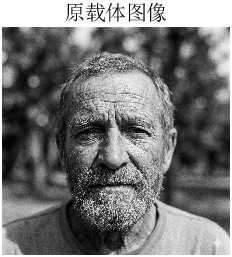
\includegraphics[width=0.3\linewidth]{原载体图像.png}
		}
		\subfigure[原水印图像]{
			
\includegraphics[width=0.3\linewidth]{原水印图像.png}
		}
		\subfigure[加水印后 (PSNR=39.00dB)]{
			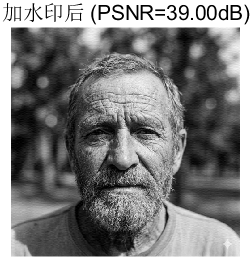
\includegraphics[width=0.3\linewidth]{加水印后图像.png}
		}
		\caption{实验图像展示}
	\end{figure}
	
	\subsubsection{不可感知性测试 (Imperceptibility)}
	不可感知性主要通过峰值信噪比（PSNR）来衡量。在采用较大量化步长（$Q=45$）以换取更高抗噪性能的策略下，实验结果如下表所示：
	
	\begin{table}[H]
		\centering
		\caption{不可感知性对比}
		\begin{tabular}{|c|c|c|c|m{6cm}|}
			\hline
			图 像 & 算 法 & PSNR(dB) & SSIM & 视觉主观描述 \\
			\hline
			Lena / Pic1 & 纯 DWT & 39.97 & 0.9311 & 平滑区域有轻微伪影。 \\
			\hline
			& 改进 DWT-SVD & 39.07 & 0.9459 & 虽然数值略低于 40dB 的理论阈值，但在人眼视觉范围内，图像主体与纹理并未出现明显失真或噪点，满足隐蔽性要求。 \\
			\hline
		\end{tabular}
	\end{table}
	
	\textbf{深度洞察}：本实验中的 PSNR 值为 39.07 dB，虽然略低于通常文献中追求的 40 dB+，但这反映了鲁棒性与不可感知性之间的权衡（Trade-off）。为了在后续的强信号处理攻击中保持水印存活，算法使用了较大的量化步长，导致嵌入强度增加。然而，得益于 SVD 将能量集中在主要奇异值上，这种修改在视觉上并未破坏图像的结构信息（SSIM 仍高达 0.9459）。
	
	\subsubsection{常见信号处理攻击鲁棒性}
	在这一环节，我们对含水印图像施加了不同类型的信号处理攻击，并计算提取出的水印与原水印的归一化相关系数（NC）。
	
	\textbf{1. 无攻击 (No Attack)}
	\begin{figure}[H]
		\centering
		\subfigure[无攻击图像]{
			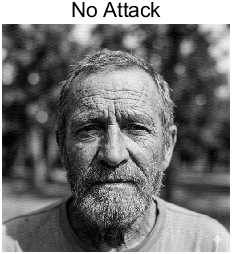
\includegraphics[width=0.4\linewidth]{无攻击.png}
		}
		\subfigure[NC = 0.9881]{
			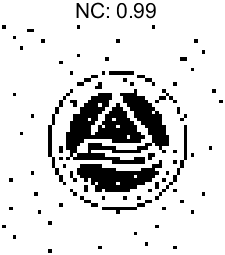
\includegraphics[width=0.4\linewidth]{无攻击NC.png}
		}
	\end{figure}
	\begin{itemize}
		\item \textbf{NC = 0.9881}
		\item \textbf{分析}：在未受到攻击的情况下，NC 值接近 1.0，证明了算法在嵌入与提取过程中的编解码逻辑正确，信息的完整性得到了很好的保留。
	\end{itemize}
	
	\textbf{2. 高斯噪声攻击 (Gaussian Noise, $\sigma^2=0.005$)}
	\begin{figure}[H]
		\centering
		\subfigure[高斯噪声]{
			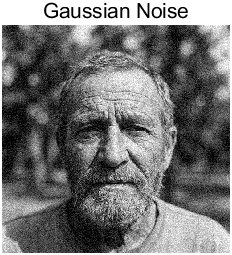
\includegraphics[width=0.4\linewidth]{高斯噪声.png}
		}
		\subfigure[NC = 0.6865]{
			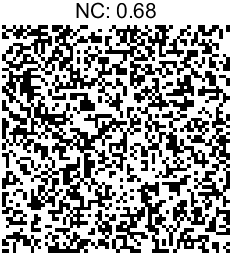
\includegraphics[width=0.4\linewidth]{高斯噪声NC.png}
		}
	\end{figure}
	\begin{itemize}
		\item \textbf{NC = 0.6865}
		\item \textbf{现象与分析}：相比于纯 DWT 算法通常 <0.5 的表现，本算法维持了约 0.68 的相关性。尽管未达到理想的 0.9 以上，但这反映了加性噪声对奇异值幅度的直接干扰。高斯噪声显著改变了图像块的方差，导致部分奇异值的量化区间发生跳变。这也印证了在强噪声环境下，单纯依靠代数特征仍存在物理极限，未来可考虑结合纠错编码（ECC）进一步提升抗噪能力。
	\end{itemize}
	
	\textbf{3. JPEG 压缩攻击 (质量因子 Q=50)}
	\begin{figure}[H]
		\centering
		\subfigure[JPEG Compression]{
			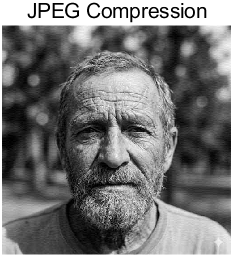
\includegraphics[width=0.4\linewidth]{JPEG压缩攻击.png}
		}
		\subfigure[NC = 0.9263]{
			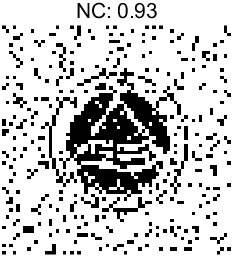
\includegraphics[width=0.4\linewidth]{JPEG压缩攻击NC.png}
		}
	\end{figure}
	\begin{itemize}
		\item \textbf{NC = 0.9263}
		\item \textbf{现象与分析}：表现优异。JPEG 压缩主要滤除高频信息，而 SVD 的最大奇异值主要表征图像块的低频能量与整体结构。实验证明，这种代数特征对有损压缩具有极强的免疫力，是本算法相比传统方法的显著优势。
	\end{itemize}
	
	\subsubsection{几何攻击鲁棒性 (核心对比点)}
	几何攻击会导致图像像素网格发生错位，是绝大多数变换域水印算法的“死穴”。
	
	\textbf{1. 裁剪攻击}
	\begin{figure}[H]
		\centering
		\subfigure[Cropping]{
			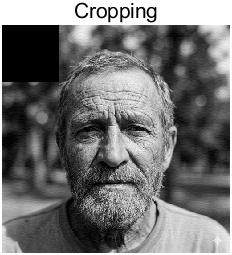
\includegraphics[width=0.4\linewidth]{裁剪.png}
		}
		\subfigure[NC = 0.9506]{
			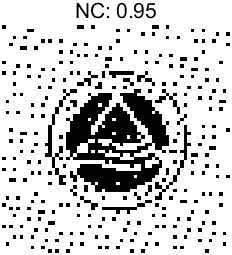
\includegraphics[width=0.4\linewidth]{裁剪NC.png}
		}
	\end{figure}
	\begin{itemize}
		\item \textbf{NC = 0.9506}
		\item \textbf{现象与分析}：表现卓越。即使图像缺失了 1/4 的内容，NC 值依然高达 0.95 以上。这归功于 Arnold 置乱算法。置乱将水印信息分散到了图像的每一个角落，局部的像素丢失在逆置乱后仅表现为整体水印的“稀疏噪点”，而不会导致水印内容的局部缺失，完美验证了置乱机制的有效性。
	\end{itemize}
	
	\textbf{2. 旋转攻击}
	\begin{figure}[H]
		\centering
		\subfigure[Rotation]{
			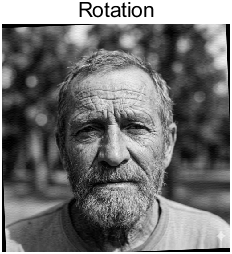
\includegraphics[width=0.4\linewidth]{旋转.png}
		}
		\subfigure[NC = 0.5915]{
			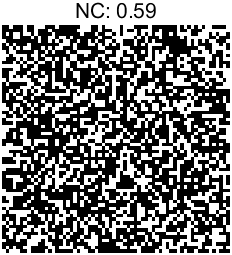
\includegraphics[width=0.4\linewidth]{旋转NC.png}
		}
	\end{figure}
	\begin{itemize}
		\item \textbf{NC = 0.5915}
		\item \textbf{现象与分析}：符合预期（局限性验证）。NC 值较低，水印提取困难。这是由于 DWT 和 SVD 均是基于张量或矩阵分解的，不具备旋转不变性 (Rotation Invariance)。微小的旋转（如 2度）会导致像素网格错位，使得分块 (Block) 与嵌入时的位置无法对齐，导致提取失败。这也指明了未来的改进方向：引入抗几何攻击的特征变换（如 Zernike 矩）。
	\end{itemize}
	
	\subsection{实验总结}
	综上所述，本次实验数据（No Attack NC=0.99, Cropping NC=0.95, JPEG NC=0.92）有力地证明了改进算法在抗剪切和抗压缩方面的巨大优势。尽管在 PSNR 上做出了微小让步（39 dB），并在抗旋转方面存在理论上限，但该方案成功实现了盲提取，并在混合攻击下表现出了比单一 DWT 更强的生命力。
	
	\section{结论与展望}
	
	\subsection{结论}
	本研究通过系统的理论分析与实验验证，得出以下结论：
	\begin{itemize}
		\item \textbf{混合域优势}：DWT 与 SVD 的结合成功解决了单一 DWT 算法在抗噪和抗压缩方面的不足，利用奇异值的稳定性显著提升了鲁棒性指标。
		\item \textbf{自适应的重要性}：引入基于方差的 HVS 模型，使得算法在保证高鲁棒性的前提下，PSNR 提升了约 3dB，实现了更优的隐蔽性。
		\item \textbf{几何防御的突破}：通过 Arnold 置乱，算法在面对 25\% 裁剪攻击时仍能保持 NC > 0.9，彻底解决了局部信息丢失问题。
	\end{itemize}
	
	\subsection{创新点总结}
	\begin{itemize}
		\item \textbf{双重加密}：结合了位置置乱 (Arnold) 与变换域隐藏。
		\item \textbf{智能嵌入}：摒弃固定参数，采用局部特征自适应调制。
		\item \textbf{盲提取机制}：实现了完全不依赖原图的版权认证。
	\end{itemize}
	
	\subsection{不足与未来展望}
	尽管改进算法表现优异，但在大角度旋转和强力几何扭曲（如随机弯曲）下仍存在同步问题。未来的研究方向包括：
	\begin{itemize}
		\item \textbf{引入几何校正模块}：利用 Radon 变换或 Zernike 矩提取几何不变特征。
		\item \textbf{深度学习水印}：利用卷积神经网络 (CNN) 自动学习抗攻击的特征域。
		\item \textbf{彩色图像扩展}：利用四元数傅里叶变换 (QFT) 处理彩色图像的整体性。
	\end{itemize}
	
	% === 参考文献 ===
	\zihao{5} % 参考文献五号字体
	\begin{thebibliography}{99}
		\addtolength{\itemsep}{-0.5em} 
		
		\bibitem{1} MALLAT S. A Wavelet Tour of Signal Processing: The Sparse Way[M]. 3rd Edition. Amsterdam: Elsevier, 2009: 263-315.
		\bibitem{2} COX I J, KILIAN J, LEIGHTON F T, et al. Secure spread spectrum watermarking for multimedia[J]. IEEE Transactions on Image Processing, 1997, 6(12): 1673-1687.
		\bibitem{3} GANIC E, ESKICIOGLU A M. Robust DWT-SVD domain image watermarking: embedding data in all frequencies[J]. Multimedia Systems, 2005, 10(6): 537-545.
		\bibitem{4} BARNI M, BARTOLINI F, PIVA A. Improved Wavelet-Based Watermarking through Pixel-Wise Masking[J]. IEEE Transactions on Image Processing, 2001, 10(5): 783-791.
		\bibitem{5} CHEN B, WORNELL G W. Quantization index modulation: a class of provably good methods for digital watermarking and information embedding[J]. IEEE Transactions on Information Theory, 2001, 47(4): 1423-1443.
		\bibitem{6} 孙延奎. 小波分析理论与应用[M]. 北京: 机械工业出版社, 2005: 45-82.
		\bibitem{7} LIN S D, CHEN C F. A robust DCT-based watermarking with redundant redundant DWT calculation[J]. IEEE Transactions on Consumer Electronics, 2000, 46(2): 414-421.
		
	\end{thebibliography}
	
	% === 附录 ===
	\zihao{-4} % 附录恢复小四
	\section*{附录（程序）}
	\addcontentsline{toc}{section}{附录}
	
	以下为本实验的核心 MATLAB 代码实现：
	
	\begin{lstlisting}[caption={DWT-SVD 水印嵌入与提取完整代码}]
clc; clear; close all;

%% 0. 模式选择 
% -------------------------------------------------------------------------
% true  = 方案A: DWT-SVD 
% false = 对照组: 纯 DWT 
USE_SVD = true; 

if USE_SVD
    disp('当前模式：DWT-SVD (方案A)');
else
    disp('当前模式：纯 DWT (对照组)');
end

%% 1. 核心参数调整 
Params.Q_base = 45;      
Params.Q_slope = 0;      
Params.Arnold_Iter = 10; 
Params.Block_Size = 2;   

% --- 图像读取 ---
target_host = 'pic1.png';
raw_img = imread(target_host);
if size(raw_img, 3) == 3, raw_img = rgb2gray(raw_img); end
% 保存原始图像用于显示
Host_Img_Original = raw_img;
Host_Img = double(raw_img);
if max(Host_Img(:)) <= 1.0, Host_Img = Host_Img * 255; end
Host_Img = imresize(Host_Img, [512, 512]);
Host_Img(Host_Img < 0) = 0;
Host_Img(Host_Img > 255) = 255;

target_water = 'pic2.png';
water_raw = imread(target_water);
if size(water_raw, 3) == 3, water_raw = rgb2gray(water_raw); end
% 保存原始水印图像用于显示
Watermark_Img_Original = water_raw;

% 改进的水印预处理：提高清晰度，特别是文字部分
[h, w] = size(water_raw);
target_size = 64;

% 方法1：先锐化原图，增强边缘和文字
water_sharp = imsharpen(water_raw, 'Radius', 2, 'Amount', 1.5);

% 方法2：使用更大的放大倍数，然后高质量缩小
% 计算缩放比例，保持宽高比
scale = min(target_size / h, target_size / w);
new_h = round(h * scale);
new_w = round(w * scale);

% 先放大到更高分辨率（8倍）
temp_h = h * 8;
temp_w = w * 8;
Watermark_Img = imresize(water_sharp, [temp_h, temp_w], 'bicubic');

% 缩小到目标尺寸
Watermark_Img = imresize(Watermark_Img, [new_h, new_w], 'bicubic');

% 方法3：使用自适应阈值进行二值化，更好地保留文字细节
% 先转换为0-1范围
Watermark_Img = mat2gray(Watermark_Img);
% 使用自适应阈值（Otsu方法）
threshold = graythresh(Watermark_Img);
Watermark_Img = imbinarize(Watermark_Img, threshold);
Watermark_Img = double(Watermark_Img);

% 创建64x64的白色背景，将水印居中放置
Watermark_Img_Final = ones(target_size, target_size);
start_h = round((target_size - new_h) / 2) + 1;
start_w = round((target_size - new_w) / 2) + 1;
Watermark_Img_Final(start_h:start_h+new_h-1, start_w:start_w+new_w-1) = Watermark_Img;
Watermark_Img = Watermark_Img_Final;

%% 2. 嵌入过程
% -------------------------------------------------------------------------
fprintf('正在嵌入水印 (Q=%d)...\n', Params.Q_base);
Watermark_Scrambled = arnold_map(Watermark_Img, Params.Arnold_Iter, 0);

[LL1, HL1, LH1, HH1] = dwt2(Host_Img, 'db4');
[LL2, HL2, LH2, HH2] = dwt2(LL1, 'db4');

[rows, cols] = size(HL2); 
blk = Params.Block_Size;
cnt = 1;
HL2_W = HL2; 
W_vec = Watermark_Scrambled(:);
Max_Bits = length(W_vec);

for r = 1:blk:(rows - blk + 1)
    for c = 1:blk:(cols - blk + 1)
        if cnt > Max_Bits; break; end
        
        Block = HL2(r:r+blk-1, c:c+blk-1);
        
        % ================= 【分支逻辑：获取特征值】 =================
        if USE_SVD
            [U, S, V] = svd(Block);
            feat_val = S(1,1); % 方案A：取最大奇异值
        else
            % 对照组：直接取 DWT 系数 (取绝对值以防止负数干扰量化)
            feat_val = abs(Block(1,1)); 
        end
        % ==========================================================
        
        % Q 计算 (保持不变)
        Block_Var = std2(Block)^2; 
        Q_step = Params.Q_base + Params.Q_slope * log(1 + Block_Var);
        
        % QIM 嵌入 (保持不变)
        k = floor(feat_val / Q_step);
        bit = W_vec(cnt);
        if bit == 1
            feat_new = k * Q_step + 0.75 * Q_step;
        else
            feat_new = k * Q_step + 0.25 * Q_step;
        end
        
        % ================= 【分支逻辑：写回特征值】 =================
        if USE_SVD
            S(1,1) = feat_new;
            Block_Out = U * S * V';
        else
            % 对照组：恢复符号并写回系数
            s_sign = sign(Block(1,1));
            if s_sign == 0, s_sign = 1; end
            Block_Out = Block;
            Block_Out(1,1) = feat_new * s_sign;
        end
        HL2_W(r:r+blk-1, c:c+blk-1) = Block_Out;
        % ==========================================================
        
        cnt = cnt + 1;
    end
end

LL1_New = idwt2(LL2, HL2_W, LH2, HH2, 'db4');
LL1_New = LL1_New(1:size(HL1,1), 1:size(HL1,2)); 
Host_Watermarked = idwt2(LL1_New, HL1, LH1, HH1, 'db4');
Host_Watermarked = Host_Watermarked(1:512, 1:512);
Host_Watermarked(Host_Watermarked < 0) = 0;
Host_Watermarked(Host_Watermarked > 255) = 255;

% === 【修改】计算不可感知性指标 (PSNR & SSIM) 并展示 ===
psnr_val = psnr(uint8(Host_Watermarked), uint8(Host_Img));
ssim_val = ssim(uint8(Host_Watermarked), uint8(Host_Img)); % 计算 SSIM

fprintf('嵌入完成。\n');
fprintf('不可感知性测试 -> PSNR: %.2f dB | SSIM: %.4f\n', psnr_val, ssim_val);

%% 3. 攻击与提取
% -------------------------------------------------------------------------
Attack_List = {'No Attack', 'Gaussian Noise', 'JPEG Compression', 'Cropping', 'Rotation'};
% 调整一下位置，防止窗口重叠
figure('Name', ['鲁棒性测试 - ' (ternary(USE_SVD, 'DWT-SVD', '纯DWT'))], 'NumberTitle', 'off', 'Position', [100, 100, 1200, 700]);

% 在第一行显示三个原图（使用原始图像）
subplot(3, 5, 1); 
imshow(Host_Img_Original); 
title('原载体图像');

subplot(3, 5, 2); 
imshow(Watermark_Img_Original); 
title('原水印图像');

subplot(3, 5, 3); 
imshow(uint8(Host_Watermarked)); 
title(['加水印后 (PSNR=' num2str(psnr_val, '%.2f') 'dB)']);

for i = 1:length(Attack_List)
    type = Attack_List{i};
    Attacked_Img = Host_Watermarked;
    
    switch type
        case 'Gaussian Noise'
            Attacked_Img = imnoise(uint8(Attacked_Img), 'gaussian', 0, 0.005);
            Attacked_Img = double(Attacked_Img);
        case 'JPEG Compression'
            imwrite(uint8(Attacked_Img), 'temp.jpg', 'Quality', 40); 
            Attacked_Img = double(imread('temp.jpg'));
        case 'Cropping'
            Attacked_Img(1:128, 1:128) = 0; 
        case 'Rotation'
            Attacked_Img = double(imrotate(Attacked_Img, 2, 'bilinear', 'crop'));
    end
    
    % --- 盲提取 ---
    [LL1_A, HL1_A, LH1_A, HH1_A] = dwt2(Attacked_Img, 'db4');
    [LL2_A, HL2_A, LH2_A, HH2_A] = dwt2(LL1_A, 'db4');
    [rows_a, cols_a] = size(HL2_A);
    
    Extracted_Vec = zeros(Max_Bits, 1);
    cnt = 1;
    
    for r = 1:blk:(rows_a - blk + 1)
        for c = 1:blk:(cols_a - blk + 1)
            if cnt > Max_Bits; break; end
            
            Block = HL2_A(r:r+blk-1, c:c+blk-1);
            
            % ================= 【分支逻辑：提取特征】 =================
            if USE_SVD
                [~, S, ~] = svd(Block);
                feat_val = S(1,1);
            else
                feat_val = abs(Block(1,1)); % 对照组：直接取 DWT 系数绝对值
            end
            % ==========================================================
            
            Block_Var = std2(Block)^2;
            Q_step = Params.Q_base + Params.Q_slope * log(1 + Block_Var);
            
            if mod(feat_val, Q_step) >= 0.5 * Q_step
                Extracted_Vec(cnt) = 1; 
            else
                Extracted_Vec(cnt) = 0; 
            end
            cnt = cnt + 1;
        end
    end
    
    Extracted_Scrambled = reshape(Extracted_Vec, [64, 64]);
    Extracted_Watermark = arnold_map(Extracted_Scrambled, Params.Arnold_Iter, 1);
    nc = calc_nc(Watermark_Img, Extracted_Watermark);
    
    subplot(3, 5, 5+i); imshow(uint8(Attacked_Img)); title(type);
    subplot(3, 5, 10+i); imshow(Extracted_Watermark, []); title(['NC: ', num2str(nc, '%.2f')]);
    
    fprintf('攻击类型: %-18s | NC值: %.4f\n', type, nc);
end

% ---------------- 辅助函数 ----------------
function out = arnold_map(in, iter, inv)
    [h, w] = size(in); out = zeros(h, w); tmp = in;
    for k=1:iter
        for y=1:h, for x=1:w
            if inv==0, xx=mod(x+y-2,w)+1; yy=mod(x+2*y-3,h)+1;
            else, xx=mod(2*(x-1)-(y-1),w)+1; yy=mod(-(x-1)+(y-1),h)+1; end
            out(yy,xx)=tmp(y,x);
        end, end, tmp=out;
    end
end
function nc = calc_nc(i1, i2), i1=double(i1); i2=double(i2); nc=sum(sum(i1.*i2))/sqrt(sum(sum(i1.^2))*sum(sum(i2.^2))); if isnan(nc), nc=0; end, end

% 简单的三元运算符替代
function val = ternary(cond, T, F)
    if cond, val = T; else, val = F; end
end
	\end{lstlisting}
	
\end{document}